\chapter{Data-driven results}\label{ch:data-driven-results}
In this section we present the results of the data-driven models, namely the convolutional neural network (CNN) and the Fourier neural operator (FNO), for solving the shallow water equations.
We analyse three main cases:
\begin{enumerate}
    \item 1D SWE with Gaussian initial conditions. 
    \item 1D linearized SWE in spherical coordinates.
    \item 2D SWE with Gaussian initial conditions.
\end{enumerate}
In each case, we evaluate the performance of the CNN and FNO models in terms of mean squared error (MSE), mean absolute error (MAE), training time and prediction time.
In addition, we analyze the models' predictions for various initial conditions and their ability to generalize to unseen data.
We also explore their capability to transfer solution aross different grid resolutions, such as transitioning from a coarse grid to a fine grid.
Finally, we examine the models' long-term predictive performance, assessing how well they maintain accuracy over extended time steps.
%We also compare the performance of the models for different values of $\sigma$, i.e., the standard deviation of the Gaussian function.
%We do this to see how the models perform for different types of initial conditions, depending how smooth or discontinuous the solution is.

In \autoref{ch:numerical_results}, we presented the results of discontinuous test cases, operating under the premise that a solver capable of handling discontinuous solutions should also perform well with smooth solutions.
In this chapter, we shift our focus to evaluating the performance of data-driven models under smooth initial conditions, as these are more representative of real-world scenarios.

\section{1D SWE with Gaussian initial conditions}
In this section, we consider the 1D shallow water equations with Gaussian initial conditions, where the data is generated as described in \autoref{sec:data_generation_fvm}.
The initial condition for the water height $h$ is given in~\eqref{eq:1D_swe_ic_gaussian} and illustrated in \autoref{fig:NN_initial_1D}.
\begin{figure}[H]
    \centering
    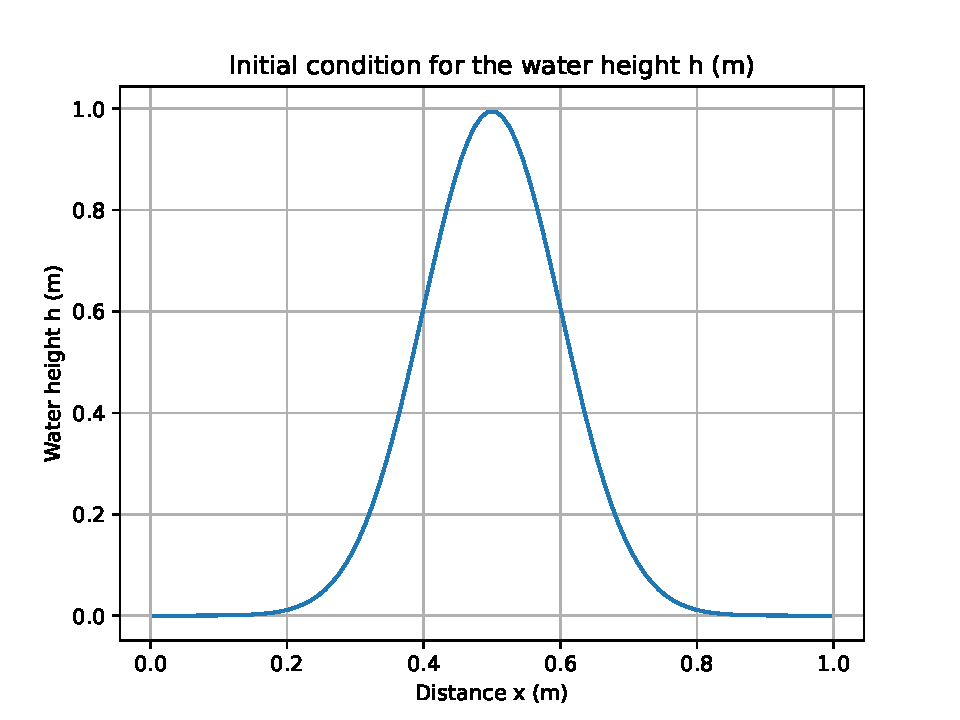
\includegraphics[width=0.5\textwidth]{C:/Users/Matteo/Shallow-Water-Equations/plots/NN_initial_1D.pdf}
    \caption{The initial conditions for water level $h$ in the 1D SWE is a Gaussian function.}\label{fig:NN_initial_1D}
\end{figure}
%The domain is $ x \in [0, 1]$ with $N = 200$ points and the final time is $t = 1.0$.
To get an overview of how the solutions evolve, we have plotted the numerical solution in the $x-t$-plane, shown in \autoref{fig:NN_initial}, in both a contour plot and a 3D plot.
\begin{figure}[H]
    %\centering
    \hspace{3cm} % Adjust the spacing as needed
    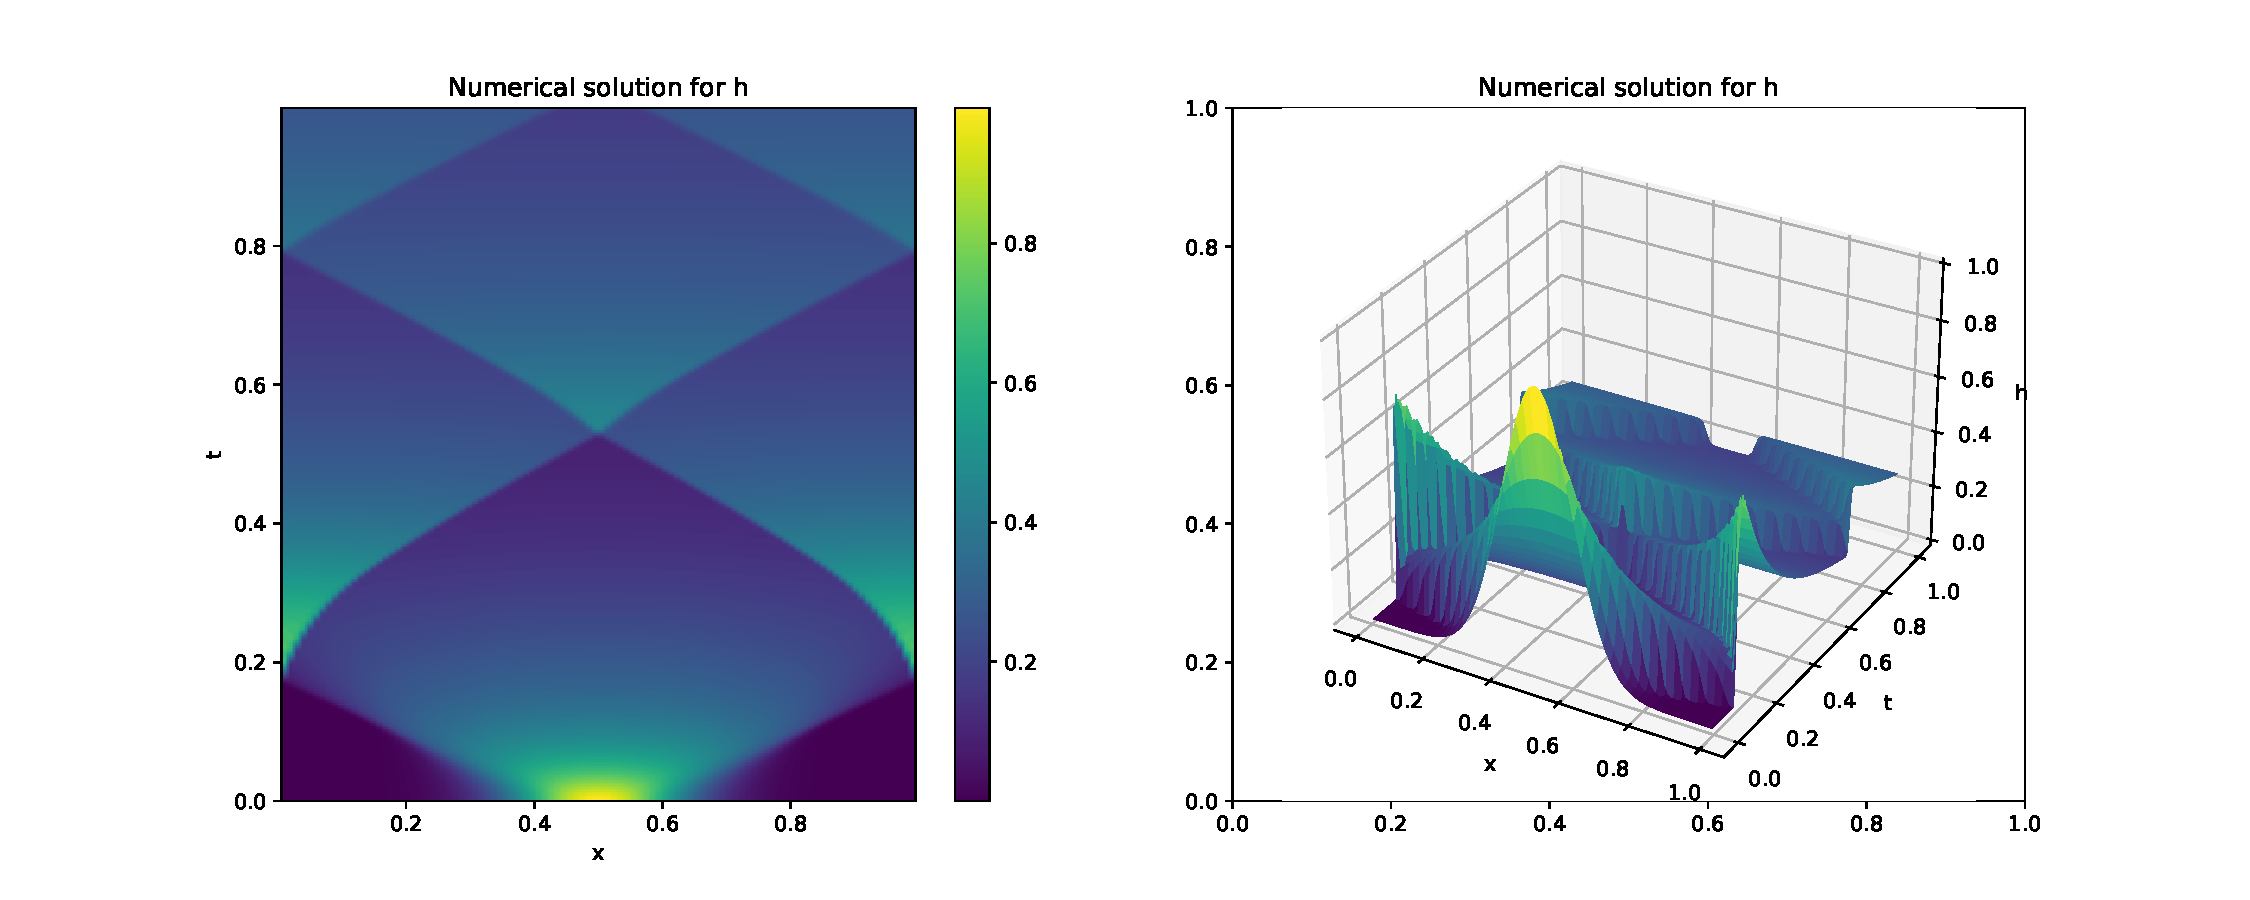
\includegraphics[width=0.8\textwidth]{C:/Users/Matteo/Shallow-Water-Equations/plots/NN_initial.pdf}
    \caption{Numerical solution of the 1D SWE from $t = 0$ s to $t = 1$ s.}\label{fig:NN_initial}
\end{figure}
In \autoref{fig:NN_initial}, we see how the solution evolves over time.
The 3d plot provides an overview of the solution, whereas the contour plot offers a more detailed view of the water level.
From the contour plot, we observe that even though the initial condition is smooth, the solution develops discontinuities over time, represented by the lines in the plot.
This behavior is typical for the nonlinear shallow water equations, where the solution can become discontinuous due to the formation of shock waves.

\subsection*{CNN Model}
%\addcontentsline{toc}{subsection}{Test case 1}
In the convolutional neural network, we train the model using the data generated by the numerical solution of the shallow water equations.
The model uses the data from the numerical solution to predict the solution at the next time step.
Meaning that the input and output data are the same, but shifted one time step. This way, the model is supposed to learn the flowmap.
The model takes input with multiple channels and applies a series of 1D convolutional layers to extract spatial features.
The model uses three convolutional layers with ReLU activation functions.
The final convolutional layer reduce the output to a single channel, and a fully connected layer maps the processed features to the output.
The model has been trained using the Adam optimizer with a learning rate of $0.001$ and a batch size of $32$.
The criteria is to minimize the mean squared error (MSE).
The model is trained on the first $60\%$ of the data, validated on the next $20\%$, and tested on the last $20\%$.
The training and validation loss for the CNN model is shown in \autoref{fig:1D_CNN_loss}.
\begin{figure}[H]
    \centering
    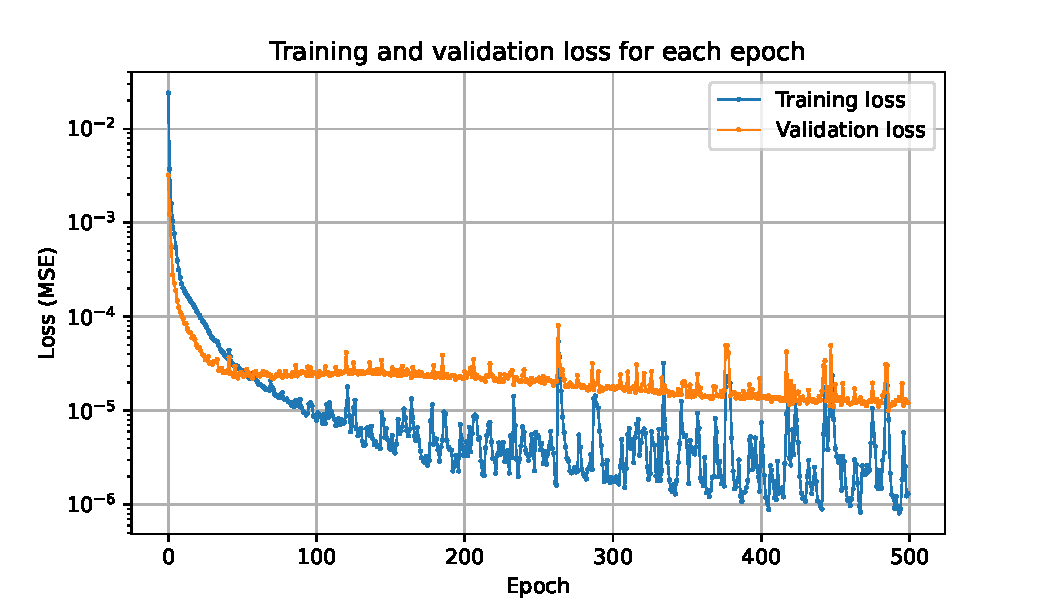
\includegraphics[width=0.7\textwidth]{C:/Users/Matteo/Shallow-Water-Equations/plots/1D_CNN_loss.pdf}
    \caption{Training and validation loss (MSE) for the CNN model.}\label{fig:1D_CNN_loss}
\end{figure}
In \autoref{fig:1D_CNN_loss}, we see that the training and validation loss decrease over the epochs, demonstrating that the model is learning the dynamics of the solution.
However, while the training loss continues to decrease, the validation loss has largely stabilized.
This indicates that further training is unlikely to improve the model's performance and may lead to overfitting.
Additionally, we assess the accuracy of the model's predictions by examining the error, as shown in \autoref{fig:1D_CNN_error}.
\begin{figure}[H]
    \centering
    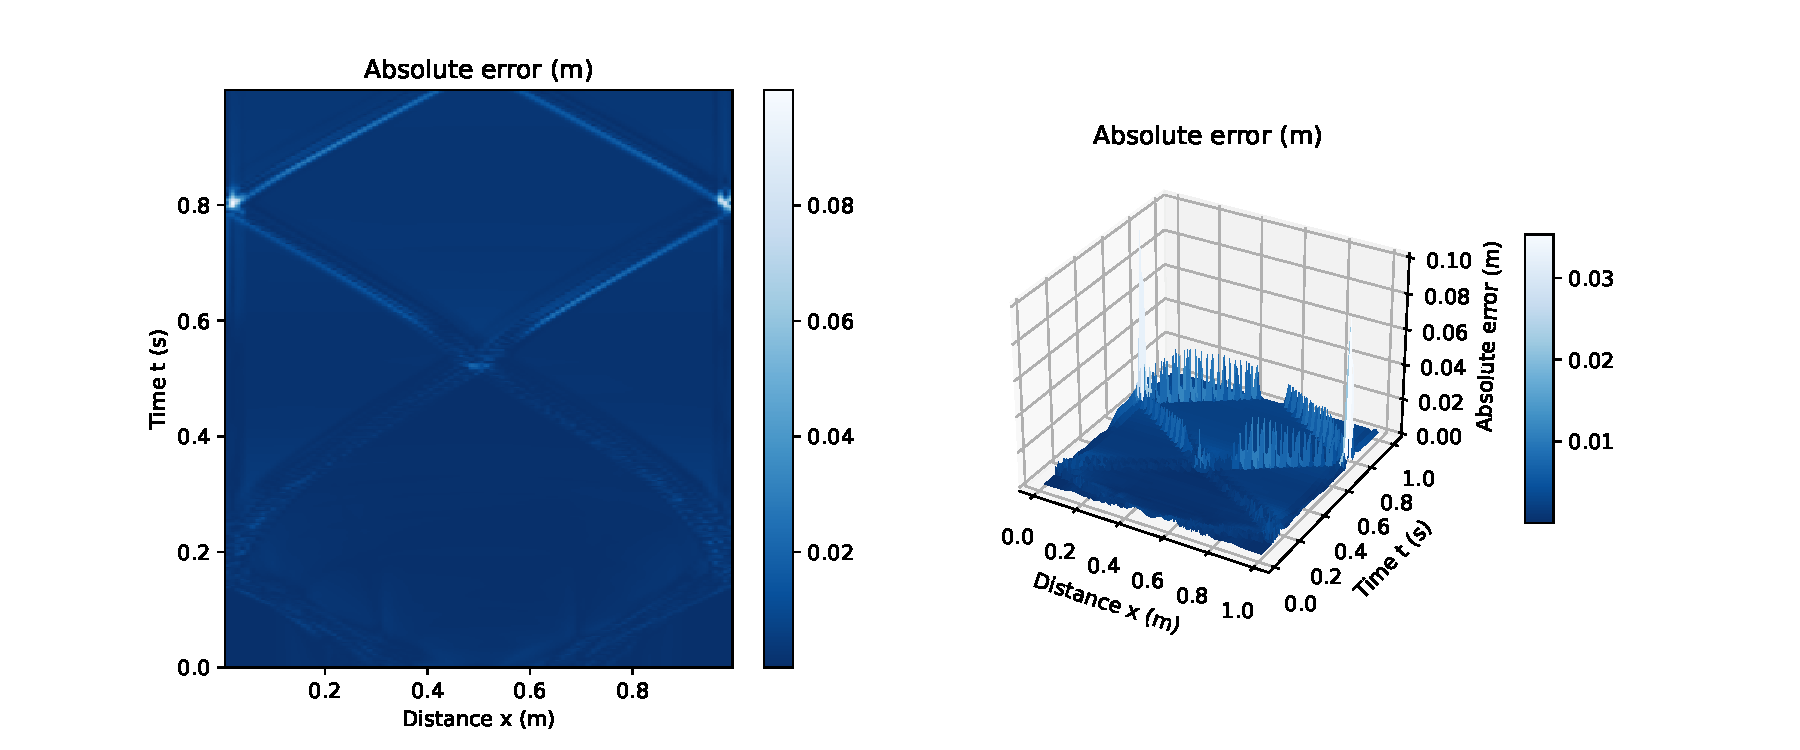
\includegraphics[width=\textwidth]{C:/Users/Matteo/Shallow-Water-Equations/plots/1D_CNN_error.pdf}
    \caption{Error plot for the predictions for the CNN model.}\label{fig:1D_CNN_error}
\end{figure}
In \autoref{fig:1D_CNN_error}, the largest errors are observed in regions where the solution exhibits discontinuities, which is expected as the model struggles to accurately predict in these areas.
We also see that, the error tends to increase over time, reflecting the model's limitations when extrapolating beyond the training data.
To gain deeper insight into the model's performance, we examine its predictions at specific time steps, as shown in \autoref{fig:1D_CNN_pred_timesteps}.
\begin{figure}[H]
    \centering
    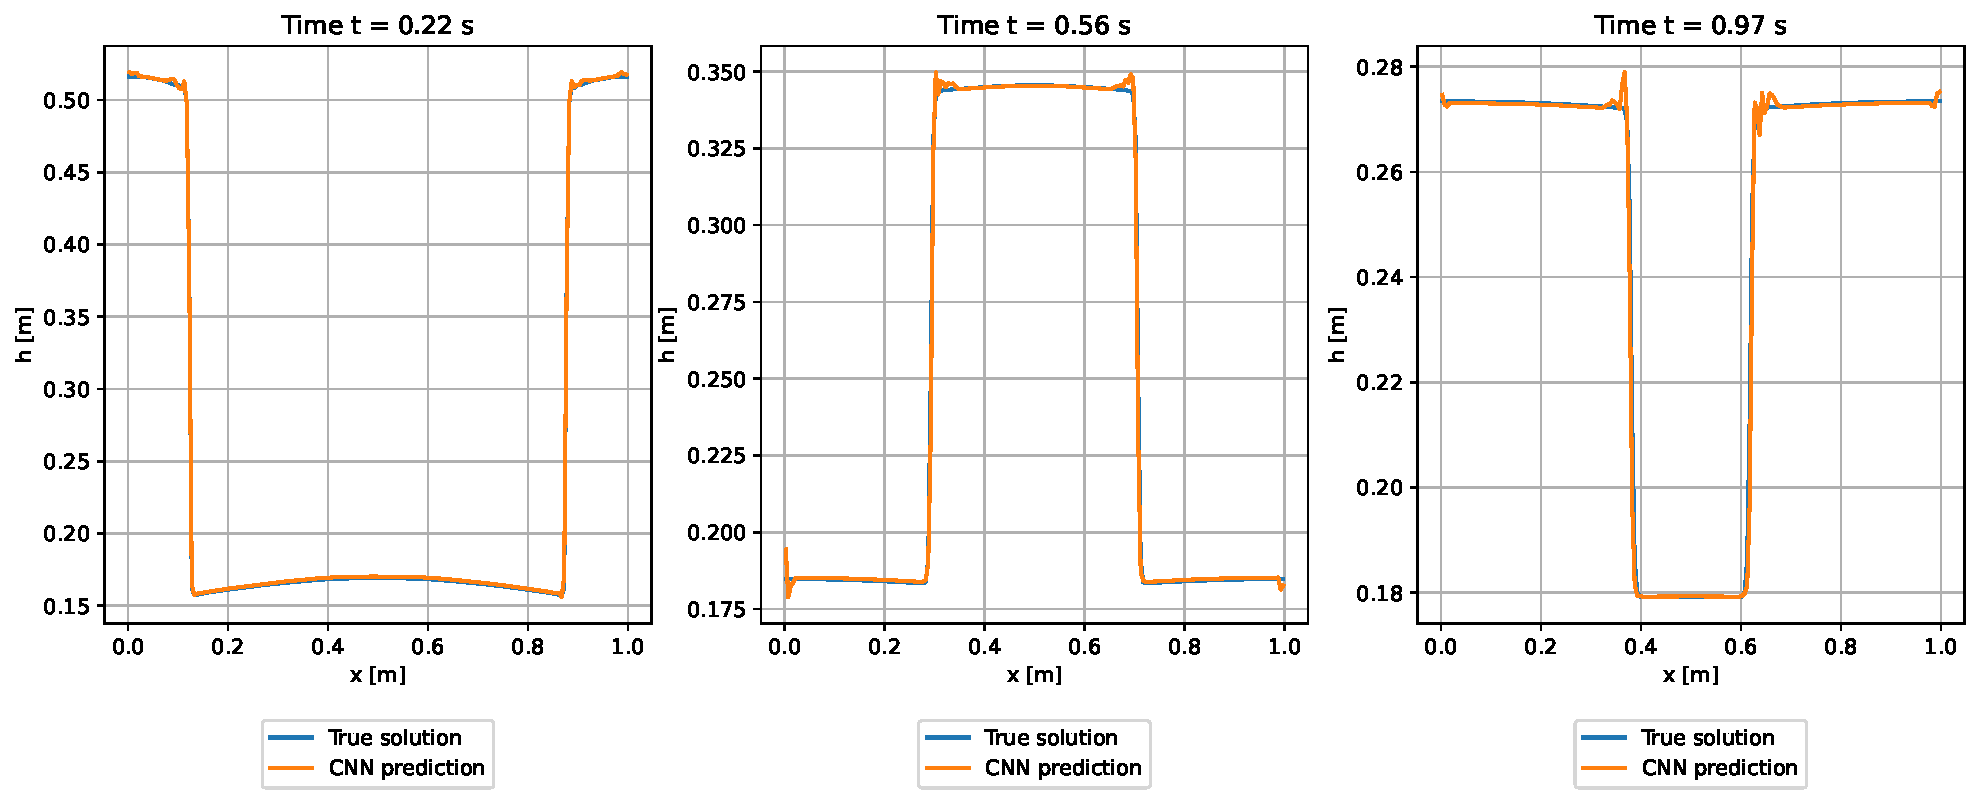
\includegraphics[width=\textwidth]{C:/Users/Matteo/Shallow-Water-Equations/plots/1D_CNN_pred_timesteps.pdf}
    \caption{Predictions for the CNN model for some given time steps.}\label{fig:1D_CNN_pred_timesteps}
\end{figure}
From \autoref{fig:1D_CNN_pred_timesteps}, we observe that the CNN model overall captures the dynamics of the solution, but struggles to predict the sharp edges.
This is expecially illustrated in the prediction at $t = 0.9$ s, where we observe oscillations in the solution that are not present in the true solution.


\subsection*{FNO Model}
We define a FNO model, which consists of an input channel, 64 hidden channels and an output channel. We use a Fourier basis with 16 modes and a batch size of 32.
The model is trained using the Adam optimizer with a learning rate of $0.001$ and the critera is to minimize the mean squared error (MSE).
We use the same train/validation/test split as for the CNN model.
The training and validation loss for the FNO model is shown in \autoref{fig:1D_FNO_loss}.
\begin{figure}[H]
    \centering
    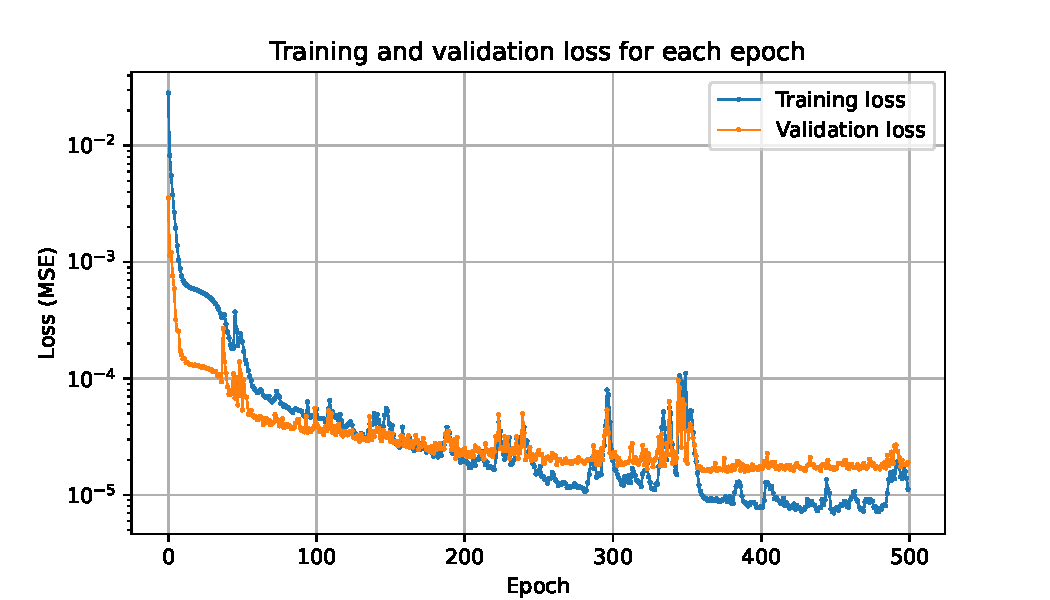
\includegraphics[width=0.7\textwidth]{C:/Users/Matteo/Shallow-Water-Equations/plots/1D_FNO_loss.pdf}
    \caption{Training and validation loss for the FNO model.}\label{fig:1D_FNO_loss}
\end{figure}
From \autoref{fig:1D_FNO_loss}, we see that the training and validation loss decrease over the epochs, indicating that the model is learning the dynamics of the solution.
As with the CNN model, the validation loss has largely stabilized, suggesting that further training is unlikely to improve the model's performance.
To see how the errors are distributed in the solution, we plot the error in \autoref{fig:1D_FNO_error}.
\begin{figure}[H]
    \centering
    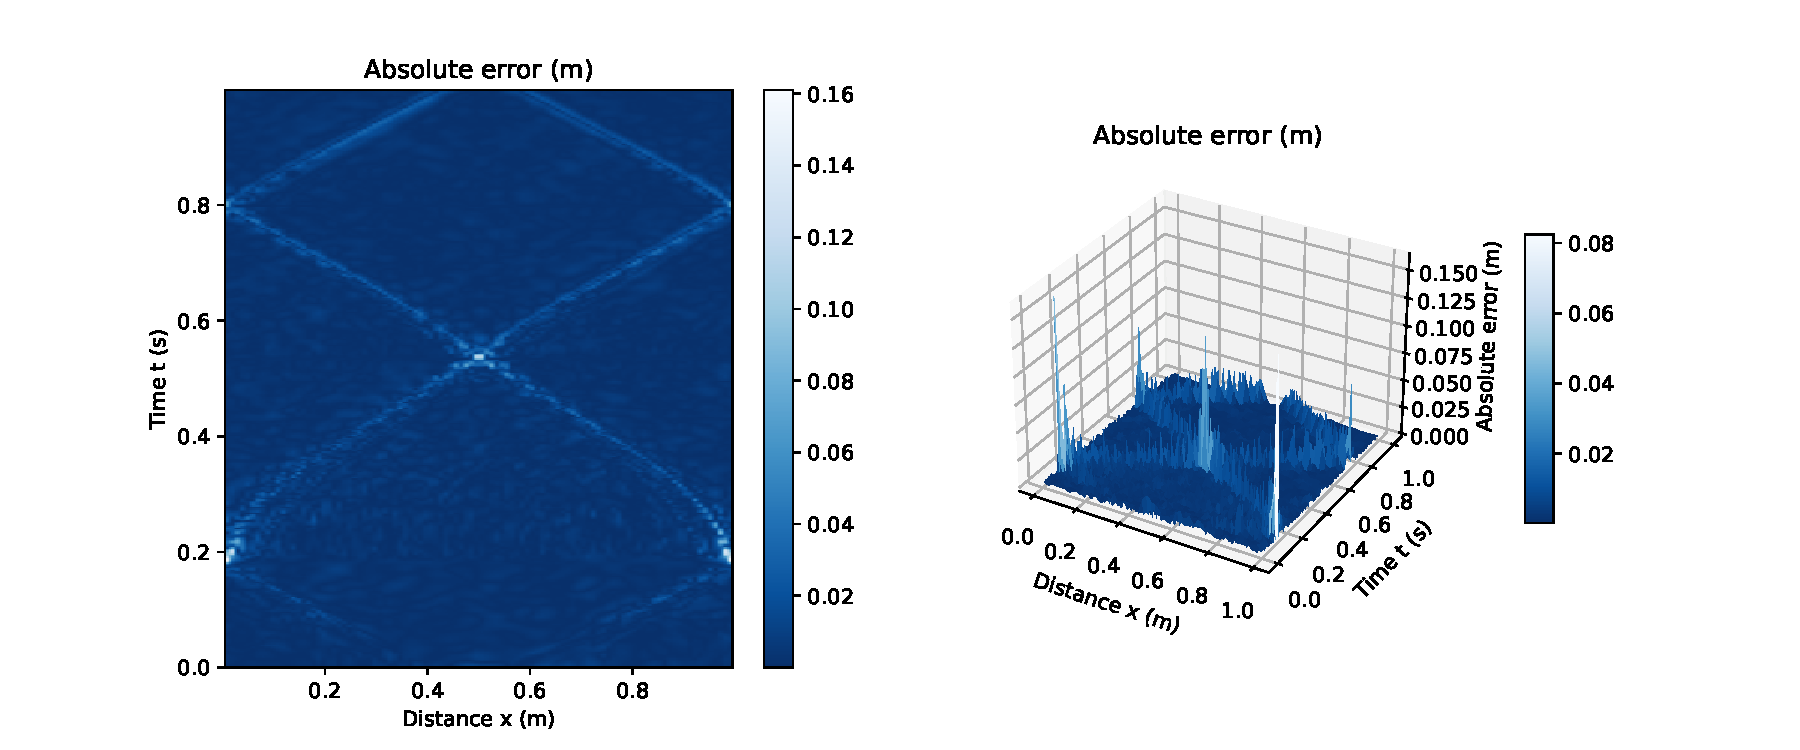
\includegraphics[width=\textwidth]{C:/Users/Matteo/Shallow-Water-Equations/plots/1D_FNO_error.pdf}
    \caption{Error plot for the predictions for the FNO model.}\label{fig:1D_FNO_error}
\end{figure}
In \autoref{fig:1D_FNO_error}, we see more or less the same error distribution as for the CNN model, with the largest errors at the discontinuities, and the error increasing over time.
To get an overview of the performance of the model, we consider the predictions for some given time steps, shown in \autoref{fig:1D_FNO_pred_timesteps}.
\begin{figure}[H]
    \centering
    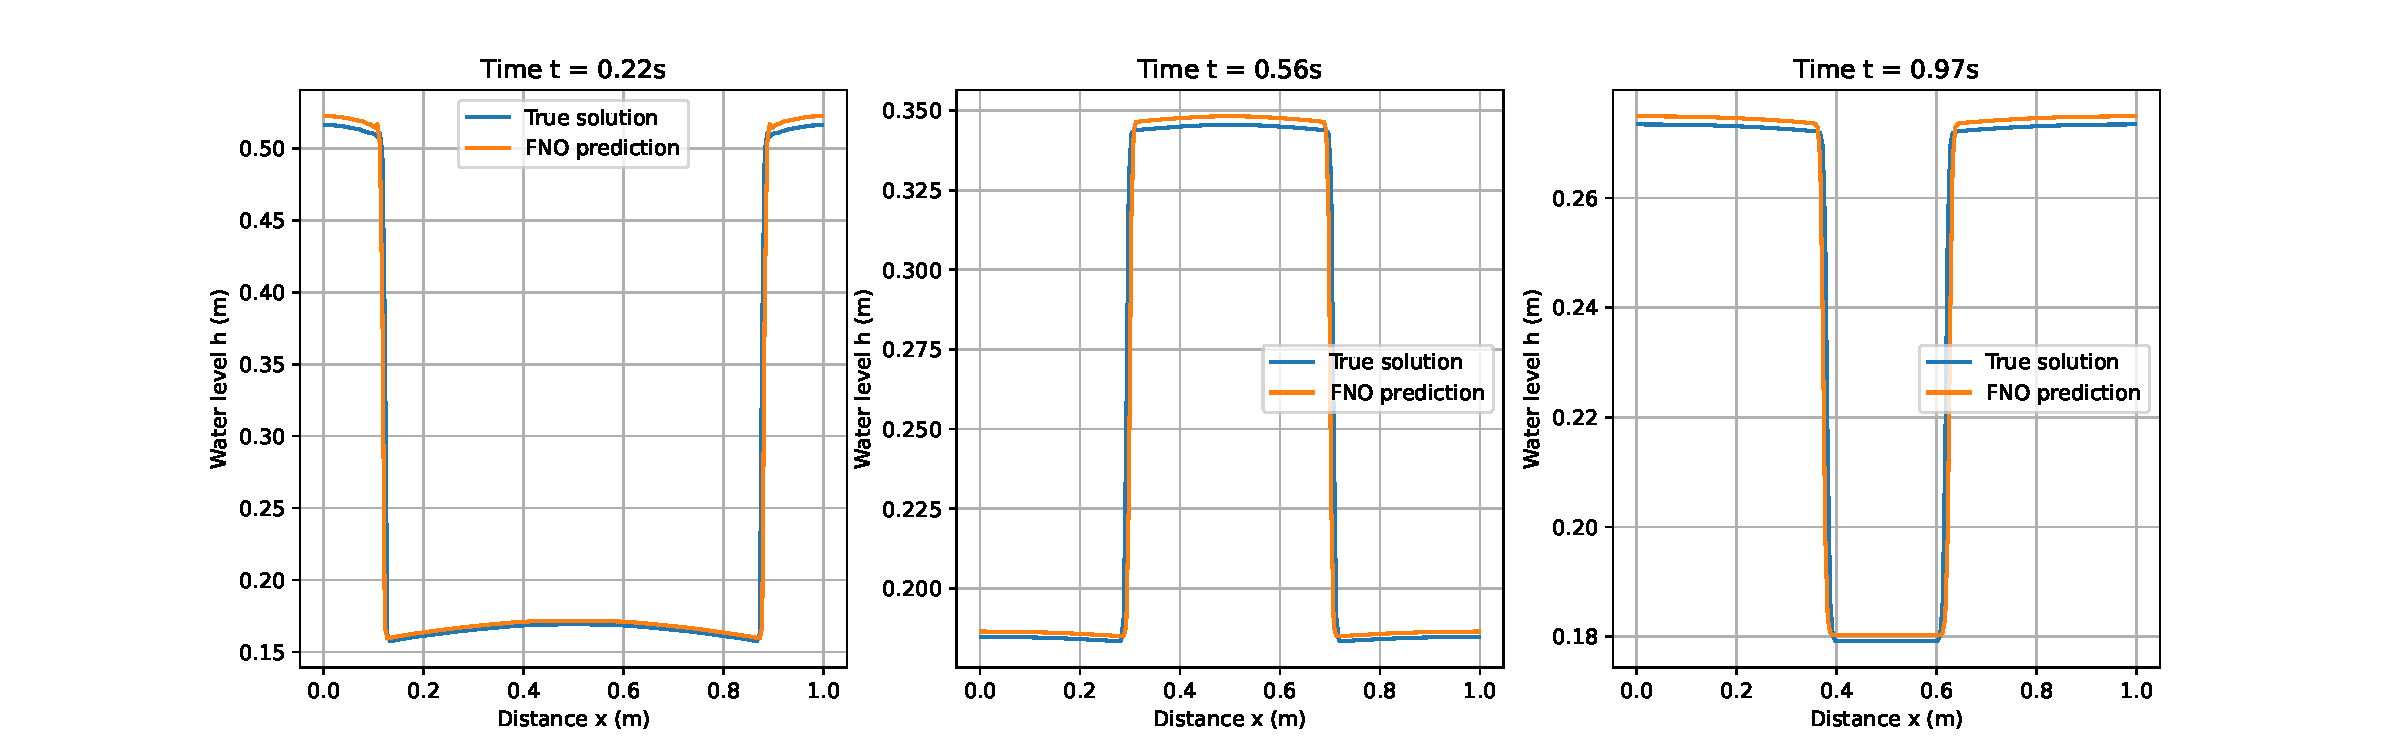
\includegraphics[width=\textwidth]{C:/Users/Matteo/Shallow-Water-Equations/plots/1D_FNO_pred_timesteps.pdf}
    \caption{Predictions for the FNO model for some given time steps.}\label{fig:1D_FNO_pred_timesteps}
\end{figure}
From \autoref{fig:1D_FNO_pred_timesteps}, we see that the FNO model overall provides a smooth and accurate prediction.

\subsection*{New initial condition}
To evaluate the models' ability to generalize to unseen initial conditions, we introduce a new initial condition for the water height $h$.
This new condition retains the Gaussian form described in~\eqref{eq:1D_swe_ic_gaussian}, but with a different mean parameter $\mu$.
Specifically, $\mu$ is set to $\mu = 0.3$ m, shifting the initial condition to the left.
The new initial condition is illustrated in \autoref{fig:1D_new_ic}.
\begin{figure}[H]
    \centering
    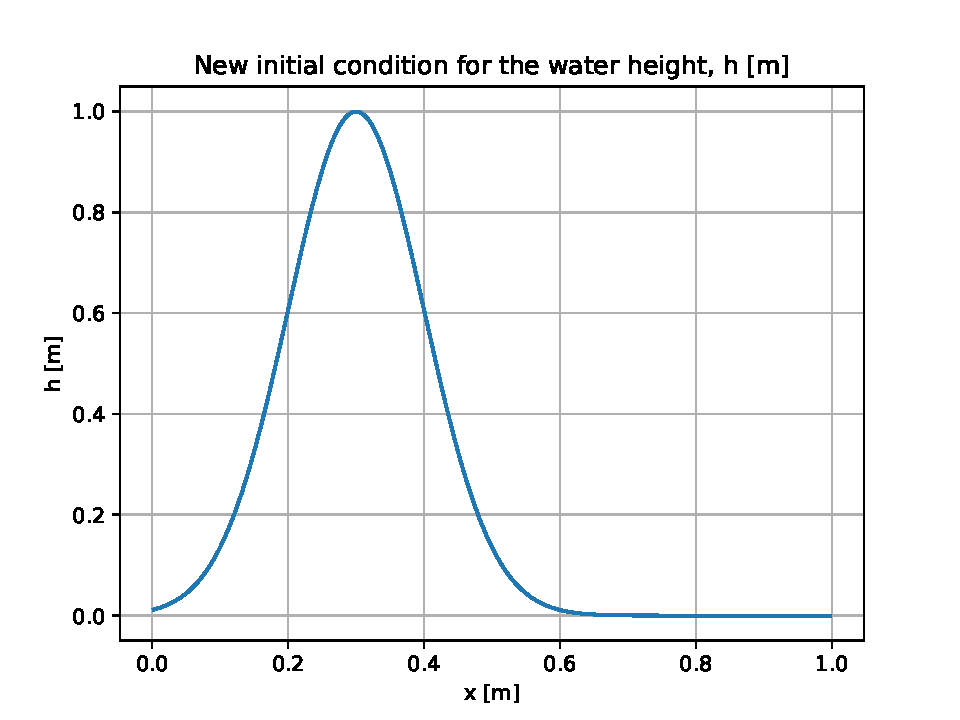
\includegraphics[width=0.5\textwidth]{C:/Users/Matteo/Shallow-Water-Equations/plots/1D_new_ic.pdf}
    \caption{New initial condition for the 1D SWE with a Gaussian function.}\label{fig:1D_new_ic}
\end{figure}
The performance of the CNN and FNO models for this new initial condition is summarized in \autoref{tab:results_1D_comparison}.
The predictions are for one time step.

\subsection*{Comparison}
To compare the performance of the CNN and FNO models, we consider the MSE and MAE for the predictions of the 1D SWE with Gaussian initial conditions.
The reason we consider both MSE and MAE is that the MSE is more sensitive to outliers, while the MAE provides a more general overview of the error.
The results are summarized in \autoref{tab:results_1D_comparison}.
\begin{table}[H]
    \centering
    \small % Reduce font size
    \begin{tabular}{c|cccc|ccc}
        Model & \multicolumn{4}{c|}{Gauss initial condition} & \multicolumn{3}{c}{New initial condition} \\
        \cline{2-8}
        & Epochs & MSE & MAE & Training time (s)  & MSE & MAE & Prediction time (s) \\
        \hline
        CNN  &
        \input{C:/Users/Matteo/Shallow-Water-Equations/saved_results/1D_CNN_nepochs.txt} &
        \input{C:/Users/Matteo/Shallow-Water-Equations/saved_results/1D_CNN_MSE_test.txt} & 
        \input{C:/Users/Matteo/Shallow-Water-Equations/saved_results/1D_CNN_MAE_test.txt} &
        \input{C:/Users/Matteo/Shallow-Water-Equations/saved_results/1D_CNN_time.txt} &
        \input{C:/Users/Matteo/Shallow-Water-Equations/saved_results/1D_CNN_MSE_test_new_ic.txt} &
        \input{C:/Users/Matteo/Shallow-Water-Equations/saved_results/1D_CNN_MAE_test_new_ic.txt} &
        \input{C:/Users/Matteo/Shallow-Water-Equations/saved_results/1D_CNN_time_new_ic.txt} 
        \\
        \hline
        FNO  &
        \input{C:/Users/Matteo/Shallow-Water-Equations/saved_results/1D_FNO_nepochs.txt} &
        \input{C:/Users/Matteo/Shallow-Water-Equations/saved_results/1D_FNO_MSE_test.txt} &
        \input{C:/Users/Matteo/Shallow-Water-Equations/saved_results/1D_FNO_MAE_test.txt} &
        \input{C:/Users/Matteo/Shallow-Water-Equations/saved_results/1D_FNO_time.txt} &
        \input{C:/Users/Matteo/Shallow-Water-Equations/saved_results/1D_FNO_MSE_test_new_ic.txt} &
        \input{C:/Users/Matteo/Shallow-Water-Equations/saved_results/1D_FNO_MAE_test_new_ic.txt} &
        \input{C:/Users/Matteo/Shallow-Water-Equations/saved_results/1D_FNO_time_newic.txt}
        \\
        \hline
    \end{tabular}
    \caption{Test loss in terms of MSE and MAE, and time for training the models for the 2D SWE.}\label{tab:results_1D_comparison}
\end{table}
From \autoref{tab:results_1D_comparison}, we see that both models has a low MSE and MAE for the Gaussian initial conditions, and hence perform well.
We note that the training time for the FNO model is significantly higher than for the CNN model.


\section{1D linearized SWE in Spherical Coordinates}
In this section, we consider the linearized shallow water equations in spherical coordinates in a 1D setting on a circular domain.
The length of the domain corresponds to the circumreference of the circle, $L = 2\pi$, and is discretized into $N = 500$ points.
The initial conditions is specified as a Gaussian function wrapped around the circle as given in~\eqref{eq:1D_swe_spherical_ic}.
We use the middle value of $\sigma$, i.e., $\sigma = \frac{\pi}{16}$, to generate the initial conditions.
The initial conditions can be seen in \autoref{fig:swe_spherical_1d_initial_conditions}.
\begin{figure}[H]
    \centering
    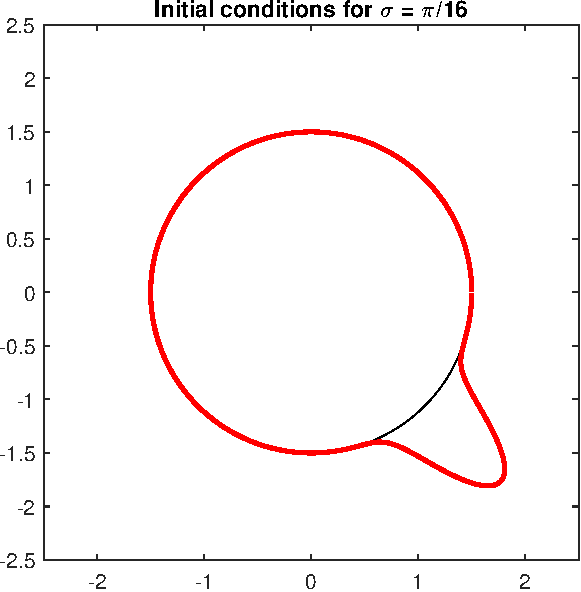
\includegraphics[width=0.4\textwidth]{C:/Users/Matteo/Shallow-Water-Equations/plots/SWE-spherical-1d-initial_conditions_sigma2.pdf}
    \caption{Initial conditions for the 1D linearized shallow water equations in spherical coordinates.}\label{fig:swe_spherical_1d_initial_conditions}
\end{figure}
To get an overview of how the solution evolves, we have plotted the numerical solution in the $\theta,t$-plane, shown in \autoref{fig:Spherical_linear_1D_true_solution}.
\begin{figure}[H]
    \centering
    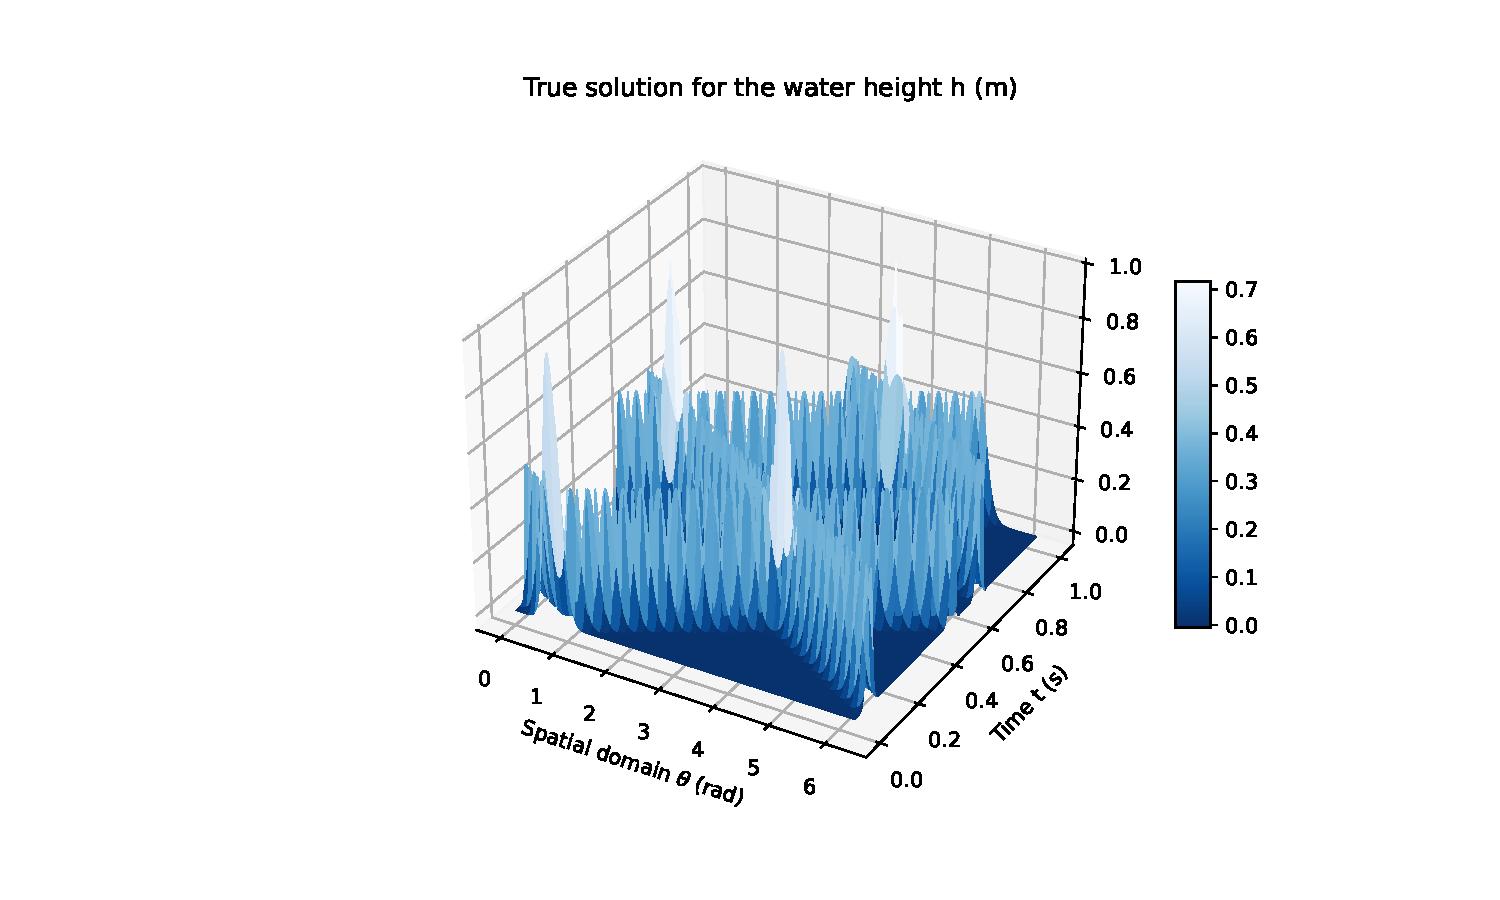
\includegraphics[width=0.8\textwidth]{C:/Users/Matteo/Shallow-Water-Equations/plots/Spherical_linear_1D_true_solution.pdf}
    \caption{Numerical solution of the spherical shallow water equations in 1D in the $\theta,t-$space.}\label{fig:Spherical_linear_1D_true_solution}
\end{figure}
In \autoref{fig:Spherical_linear_1D_true_solution}, we see that the solution has some steep descents, and it is interesting to see how the data-driven models handle these sharp edges.

\subsubsection*{CNN Model}
Ww define and train a CNN model to solve the 1D linearized shallow water equations (LSWE) in spherical coordinates.
%The model is trained on $500$ epochs.
The CNN model is trained on the data from $t = 0$ to $t = 0.6$ s, validated on the data from $t = 0.6$ to $t = 0.8$, and tested on the data from $t = 0.8$ to $t = 1.0$ s.
The training and validation loss is shown in \autoref{fig:1D_CNN_sphere_loss}.
\begin{figure}[H]
    \centering
    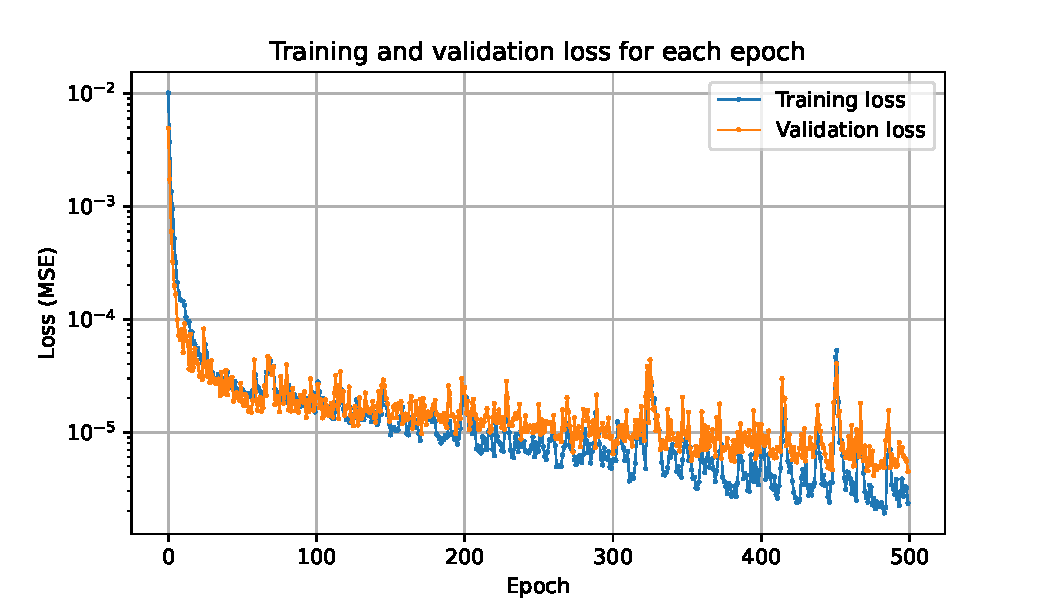
\includegraphics[width=0.7\textwidth]{C:/Users/Matteo/Shallow-Water-Equations/plots/1D_CNN_sphere_loss.pdf}
    \caption{Training and validation loss for the CNN model for the 1D spherical LSWE.}\label{fig:1D_CNN_sphere_loss}
\end{figure}
To see how the model performs, we consider the error plots in \autoref{fig:1D_CNN_sphere_error}.
\begin{figure}[H]
    \centering
    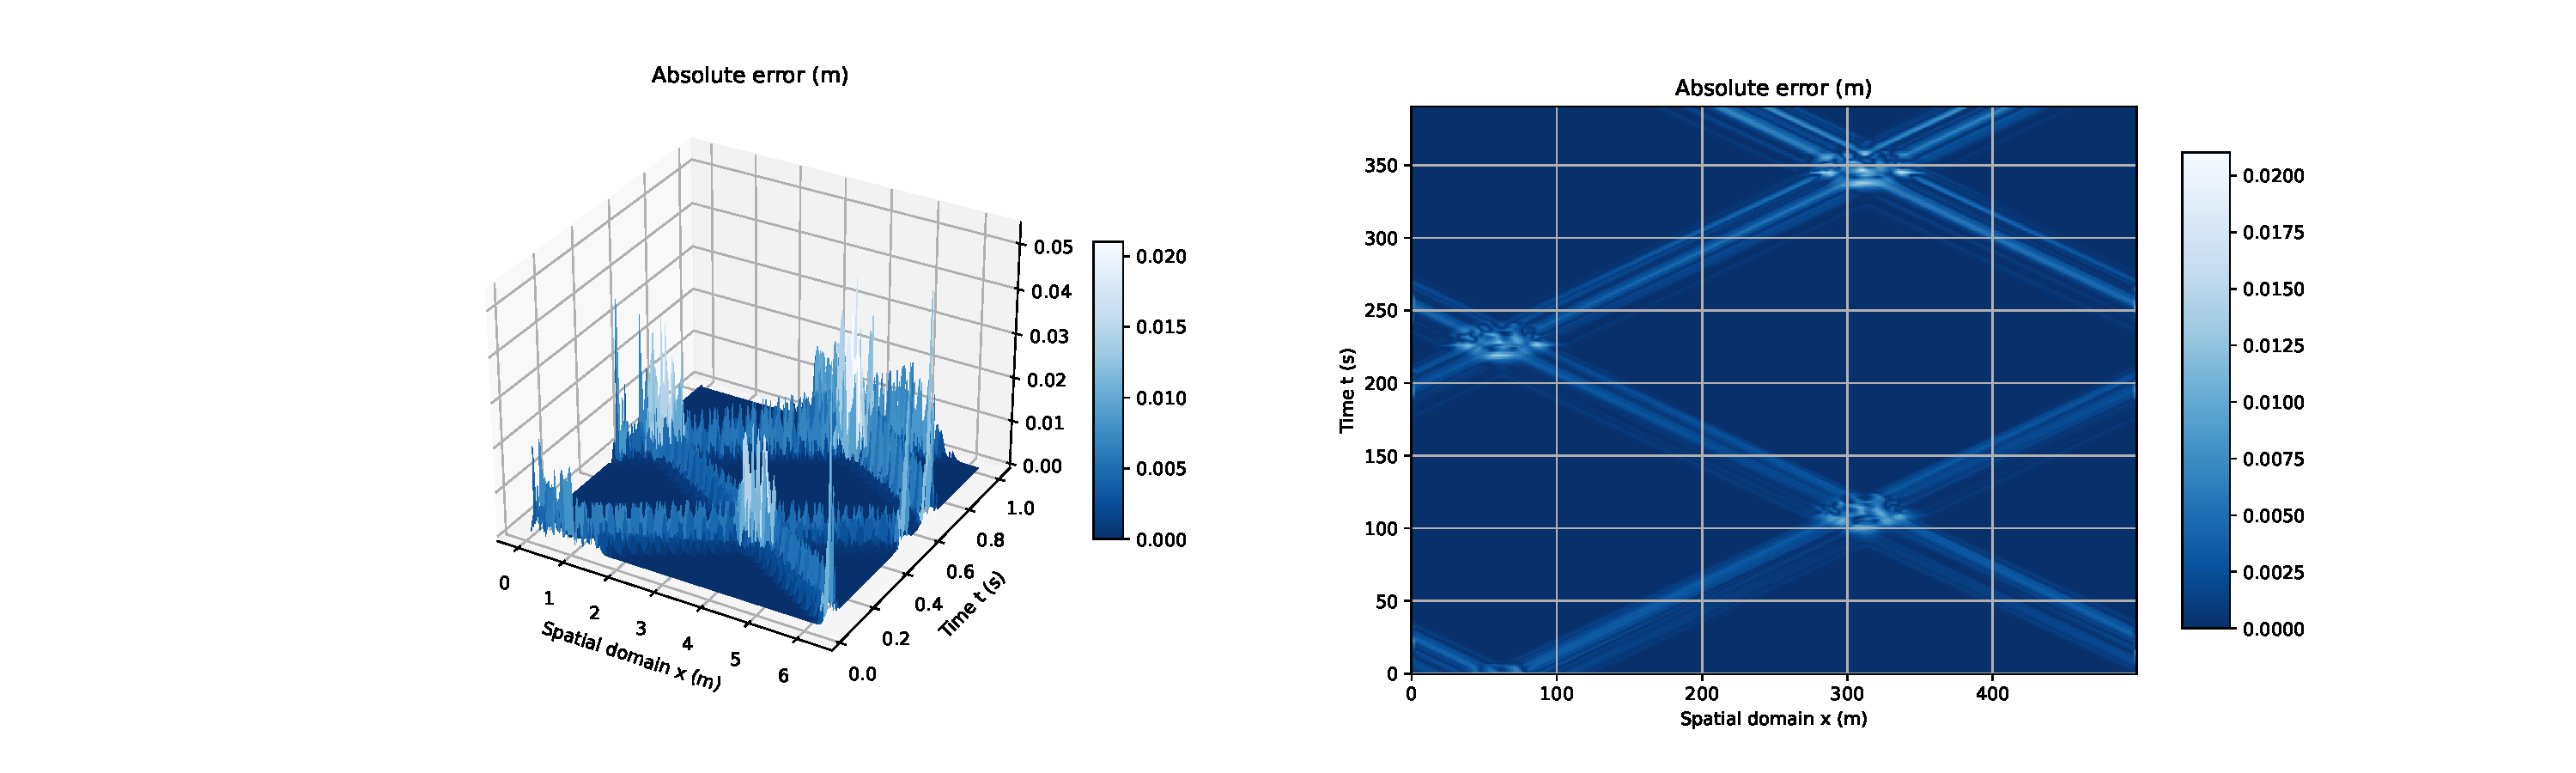
\includegraphics[width=\textwidth]{C:/Users/Matteo/Shallow-Water-Equations/plots/1D_CNN_sphere_error_sigma=2.pdf}
    \caption{Error plots for the predictions of the CNN model for solving the 1D linearized spherical SWE.}\label{fig:1D_CNN_sphere_error}
\end{figure}
In \autoref{fig:1D_CNN_sphere_error}, we see that errors are largest at the sharp edges of the solution, which is expected as the solution tends to be discontinuous.
The predictions for some given time steps are shown in \autoref{fig:1D_CNN_sphere_pred_timesteps_sphere_sigma=2}.
\begin{figure}[H]
    \centering
    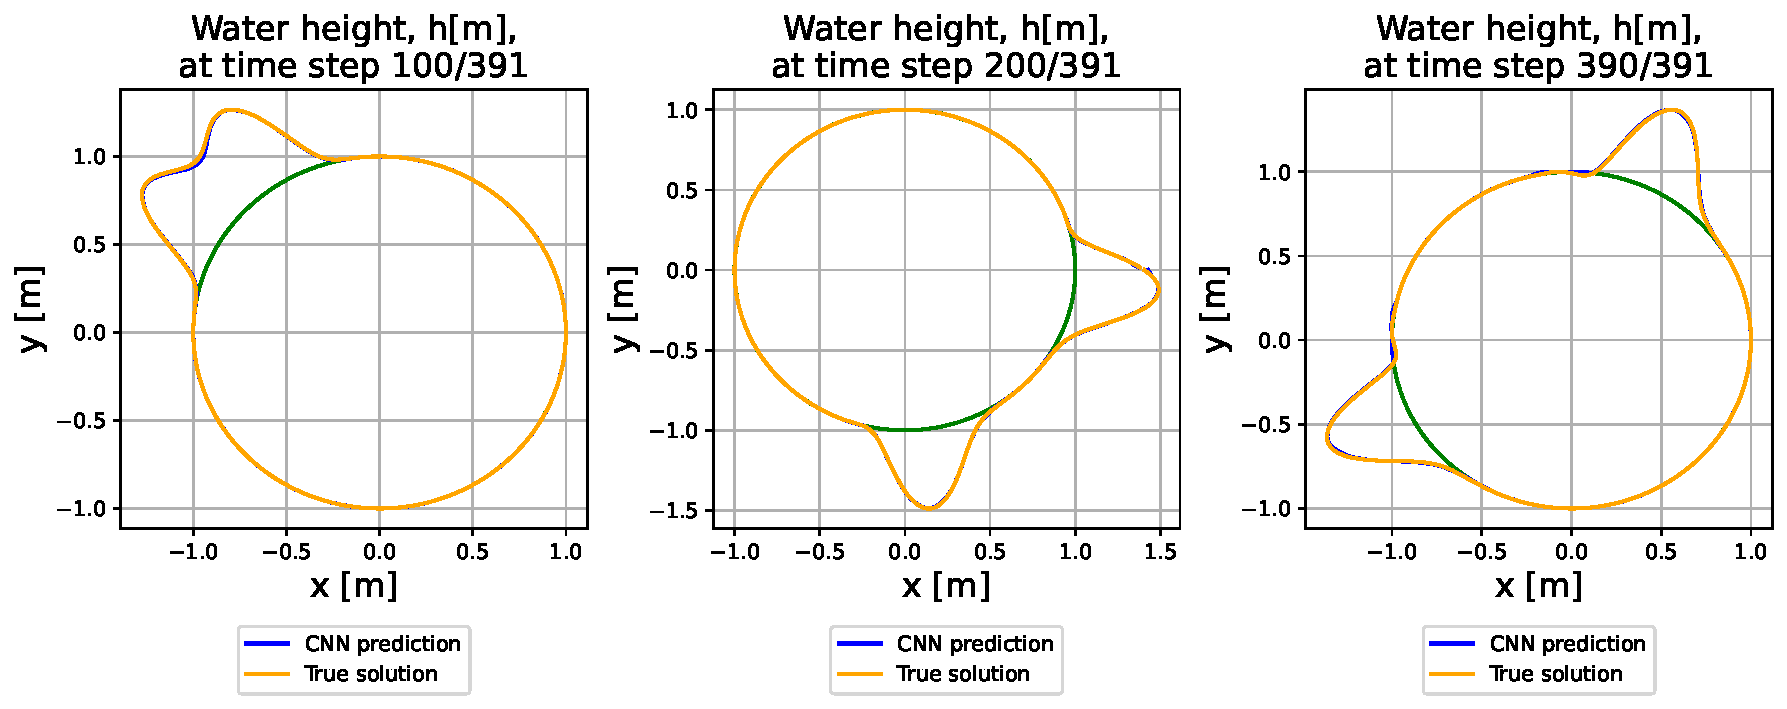
\includegraphics[width=0.9\textwidth]{C:/Users/Matteo/Shallow-Water-Equations/plots/1D_CNN_sphere_pred_timesteps_sphere_sigma=2.pdf}
    \caption{Predictions for the spherical shallow water equations in 1D using the CNN model for some given time steps.}\label{fig:1D_CNN_sphere_pred_timesteps_sphere_sigma=2}
\end{figure}
From \autoref{fig:1D_CNN_sphere_pred_timesteps_sphere_sigma=2}, we see that the predictions capture the waves, but have some over- or underestimations at the top or bottom of the waves, meaning that numerical dispersion effects are visible.



\subsubsection*{FNO model}
The FNO model consists of an input channel, 64 hidden channels and an output channel. We use a Fourier basis with 16 modes and a batch size of 32.
The model is trained using the Adam optimizer with a learning rate of $0.001$ and the critera is to minimize the mean squared error (MSE).
The model is trained on the data from $t = 0$ s to $t = 0.6$ s, validated on the data from $t = 0.6$ s to $t = 0.8$ s, and tested on the data from $t = 0.8$ s to $t = 1.0$ s.
The training and validation loss is shown in \autoref{fig:1D_FNO_sphere_loss}.
\begin{figure}[H]
    \centering
    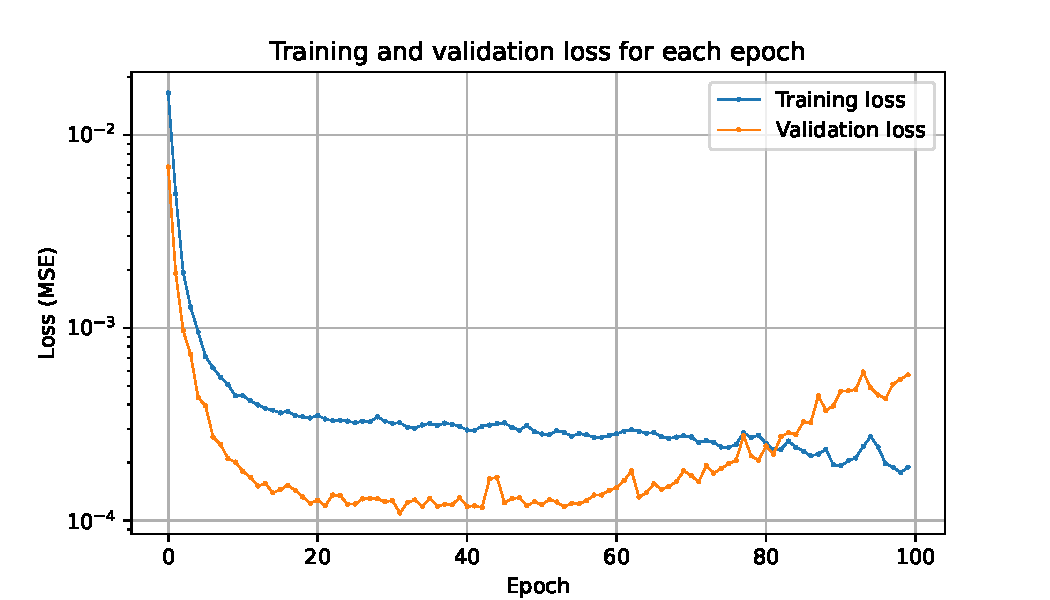
\includegraphics[width=0.7\textwidth]{C:/Users/Matteo/Shallow-Water-Equations/plots/1D_FNO_sphere_loss.pdf}
    \caption{Training and validation loss for the FNO model for the spherical shallow water equations in 1D.}\label{fig:1D_FNO_sphere_loss}
\end{figure}
\autoref{fig:1D_FNO_sphere_loss} shows that the training and validation loss decrease over the epochs, indicating that the model is learning the dynamics of the solution.
We see that after some time the validation loss increases, indicating that the model is overfitting the training data.
%We note that the cross between the training and validation loss is later, compared to the CNN model, indicating that the FNO model needs more epochs to converge.
The error plots are shown in \autoref{fig:1D_FNO_sphere_error_sigma=2}.
\begin{figure}[H]
    \centering
    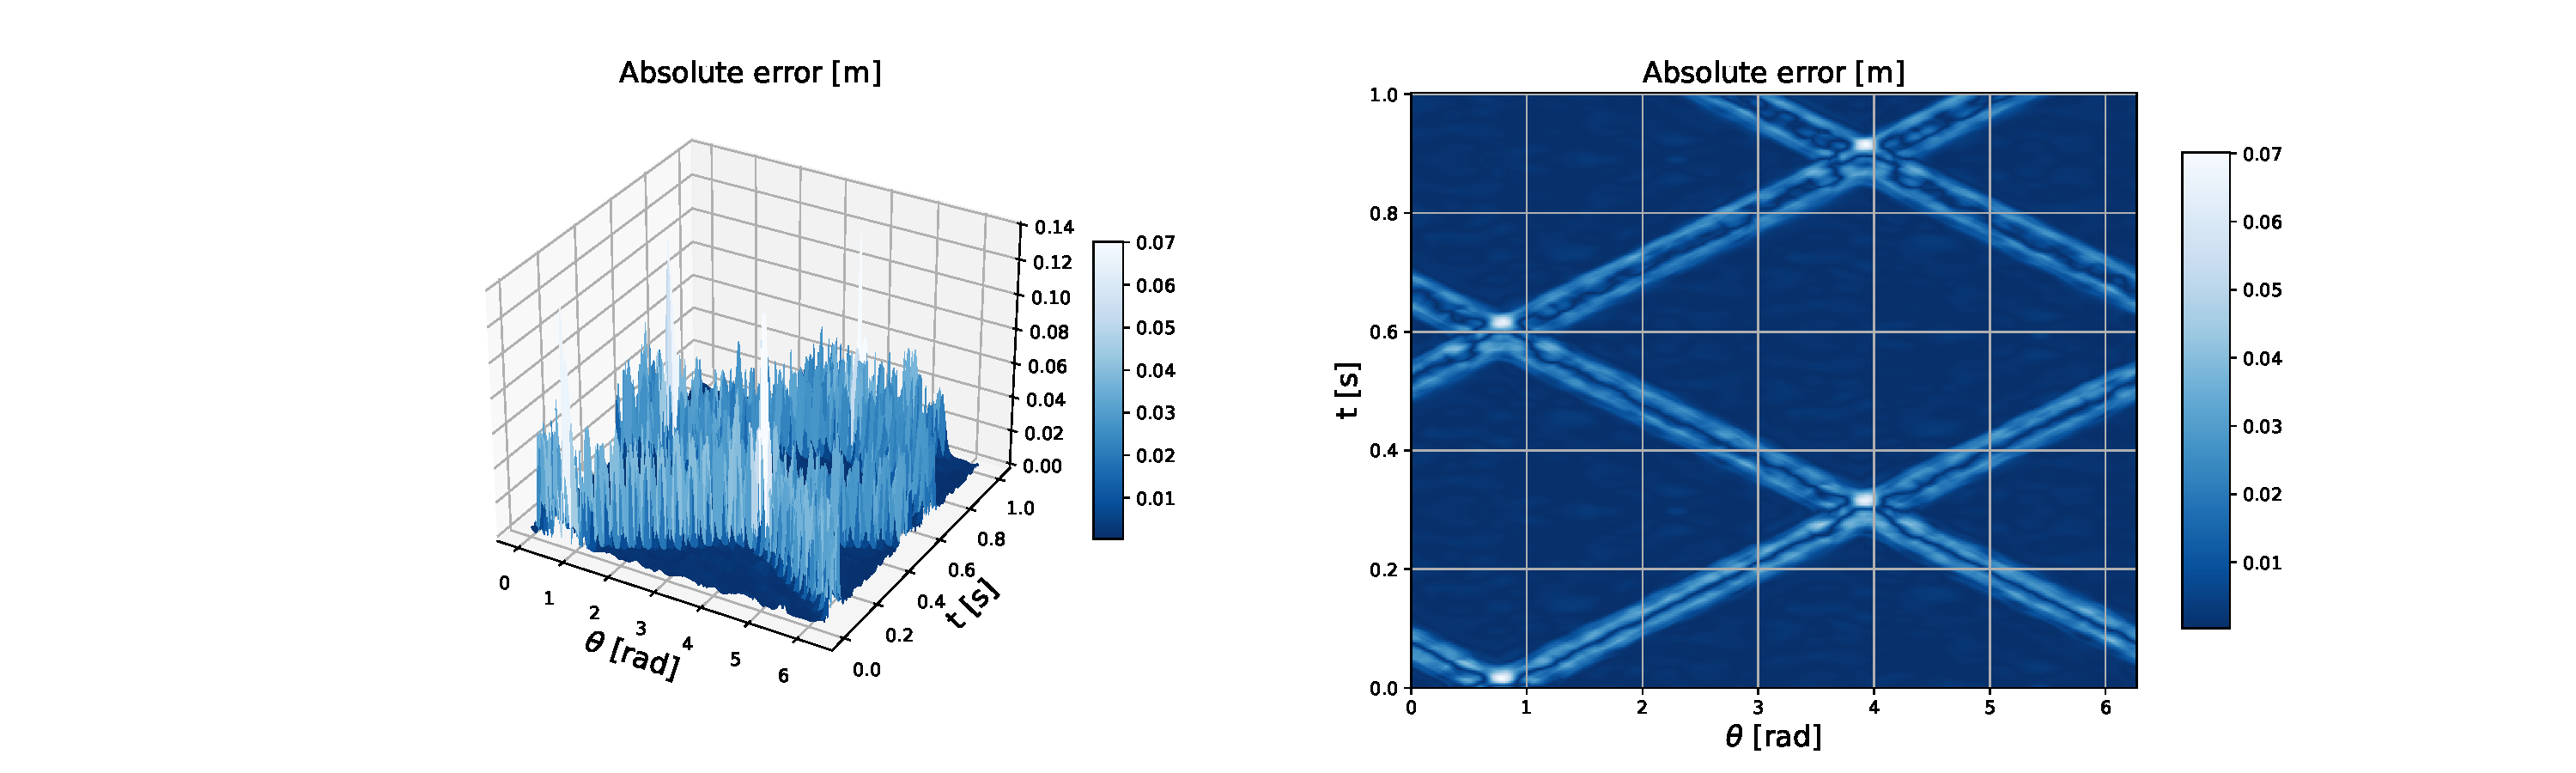
\includegraphics[width=\textwidth]{C:/Users/Matteo/Shallow-Water-Equations/plots/1D_FNO_sphere_error_sigma=2.pdf}
    \caption{Error plots for the predictions of the 1D linearized spherical SWE.}\label{fig:1D_FNO_sphere_error_sigma=2}
\end{figure}
Similar to the CNN model, we observe from \autoref{fig:1D_FNO_sphere_error_sigma=2} that the error is largest at the sharp edges of the solution.
Furthermore, the plots also indicate that the error increases over time.
This is somehow expected, as the model is trained on a limited time interval and may struggle to generalize to unseen data.
The predictions for some given time steps are shown in \autoref{fig:1D_FNO_sphere_pred_timesteps_sphere_sigma=2}.
\begin{figure}[H]
    \centering
    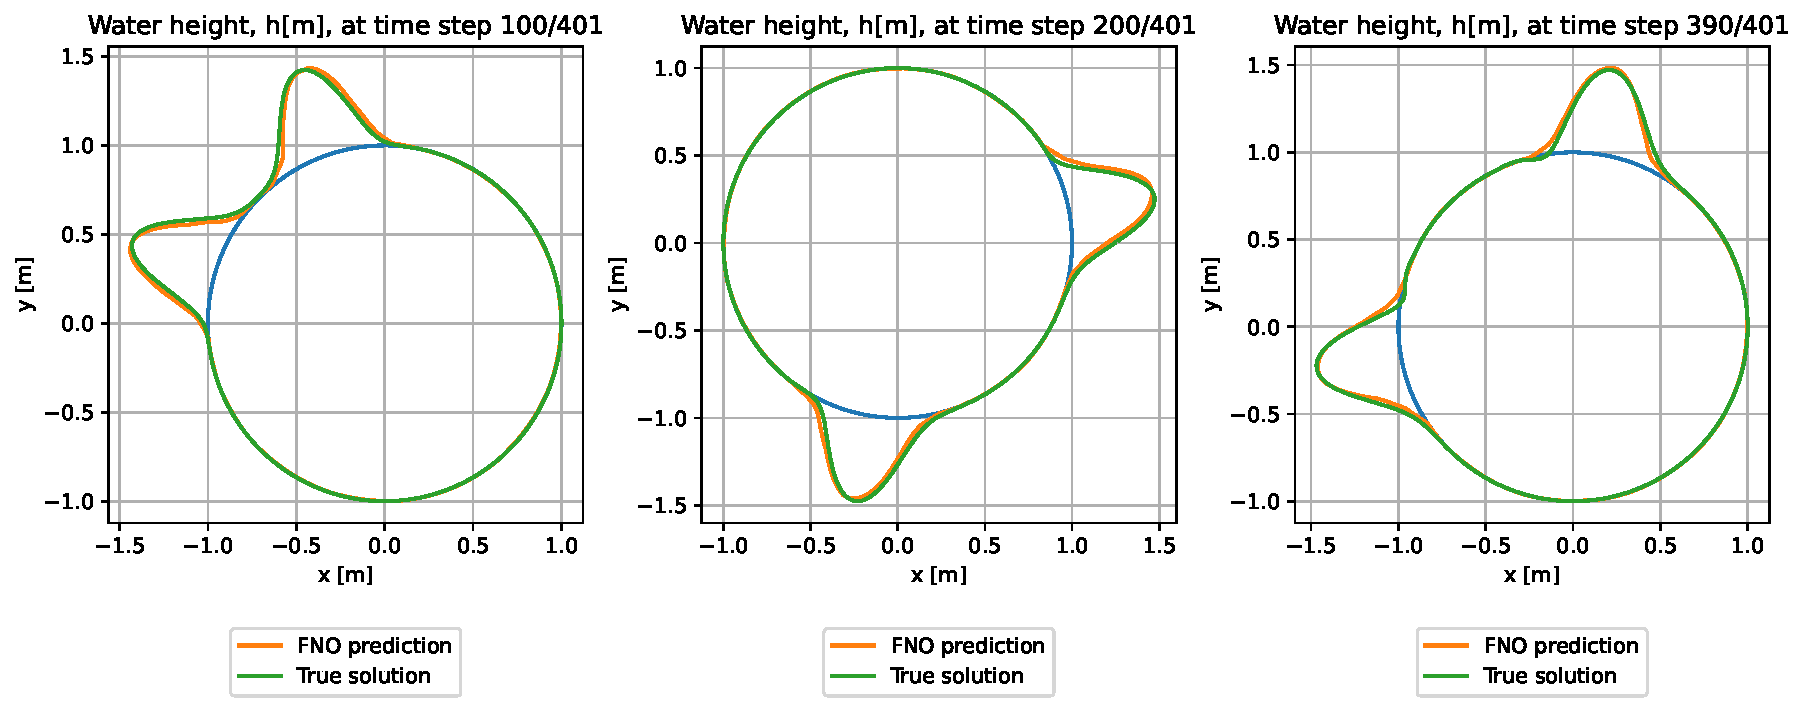
\includegraphics[width=0.9\textwidth]{C:/Users/Matteo/Shallow-Water-Equations/plots/1D_FNO_sphere_pred_timesteps_sphere_sigma=2.pdf}
    \caption{Predictions for the spherical shallow water equations in 1D using the FNO model for some given time steps.}\label{fig:1D_FNO_sphere_pred_timesteps_sphere_sigma=2}
\end{figure}
The two first plots of \autoref{fig:1D_FNO_sphere_pred_timesteps_sphere_sigma=2} shows that the FNO model captures the waves really well, but in the last plot we see that the model has some challenges, and for instance is predicting a small wave that is not present in the true solution.

\subsubsection*{Comparison}
We use the MSE and MAE to compare the performance of the CNN and FNO models for the 1D spherical LSWE.
In addition, to the results just presented, we have also trained the models for $\sigma = \frac{\pi}{8}$ and $\sigma = \frac{\pi}{32}$.
This is done to see how the models perform for different types of initial conditions, depending on how smooth or discontinuous the solution is.
The error plots and predictions for given time steps can be found in Appendix \autoref{app:1D_SWE_spherical_CNN_FNO}.
The results are summarized in \autoref{tab:results_spherical_1D_comparison}.
\begin{table}[H]
    \centering
    \small % Reduce font size
    \begin{tabular}{c|ccc|ccc|ccc}
        \hline

        Model & \multicolumn{3}{c|}{$\sigma = \pi/8$} & \multicolumn{3}{c|}{$\sigma = \pi/16$} & \multicolumn{3}{c}{$\sigma = \pi/32$} \\
        \cline{2-10}
        & MSE & MAE & Time (s) & MSE & MAE & Time (s) & MSE & MAE & Time (s) \\
        \hline
        CNN & 
        \input{C:/Users/Matteo/Shallow-Water-Equations/saved_results/1D_CNN_sphere_sigma=1_MSE_test.txt} &
        \input{C:/Users/Matteo/Shallow-Water-Equations/saved_results/1D_CNN_sphere_sigma=1_MAE_test.txt} &
        \input{C:/Users/Matteo/Shallow-Water-Equations/saved_results/1D_CNN_sphere_sigma=1_time.txt} &
        \input{C:/Users/Matteo/Shallow-Water-Equations/saved_results/1D_CNN_sphere_sigma=2_MSE_test.txt} &
        \input{C:/Users/Matteo/Shallow-Water-Equations/saved_results/1D_CNN_sphere_sigma=2_MAE_test.txt} &
        \input{C:/Users/Matteo/Shallow-Water-Equations/saved_results/1D_CNN_sphere_sigma=2_time.txt} &
        \input{C:/Users/Matteo/Shallow-Water-Equations/saved_results/1D_CNN_sphere_sigma=3_MSE_test.txt} &
        \input{C:/Users/Matteo/Shallow-Water-Equations/saved_results/1D_CNN_sphere_sigma=3_MAE_test.txt} &
        \input{C:/Users/Matteo/Shallow-Water-Equations/saved_results/1D_CNN_sphere_sigma=3_time.txt}
        \\ 
        \hline
        FNO & 
        \input{C:/Users/Matteo/Shallow-Water-Equations/saved_results/1D_FNO_sphere_sigma=1_MSE_test.txt} &
        \input{C:/Users/Matteo/Shallow-Water-Equations/saved_results/1D_FNO_sphere_sigma=1_MAE_test.txt} &
        \input{C:/Users/Matteo/Shallow-Water-Equations/saved_results/1D_FNO_sphere_sigma=1_time.txt} &
        \input{C:/Users/Matteo/Shallow-Water-Equations/saved_results/1D_FNO_sphere_sigma=2_MSE_test.txt} &
        \input{C:/Users/Matteo/Shallow-Water-Equations/saved_results/1D_FNO_sphere_sigma=2_MAE_test.txt} &
        \input{C:/Users/Matteo/Shallow-Water-Equations/saved_results/1D_FNO_sphere_sigma=2_time.txt} &
        \input{C:/Users/Matteo/Shallow-Water-Equations/saved_results/1D_FNO_sphere_sigma=3_MSE_test.txt} &
        \input{C:/Users/Matteo/Shallow-Water-Equations/saved_results/1D_FNO_sphere_sigma=3_MAE_test.txt} &
        \input{C:/Users/Matteo/Shallow-Water-Equations/saved_results/1D_FNO_sphere_sigma=3_time.txt}
        \\ 
        \hline
    \end{tabular}
    \caption{Test loss in terms of MSE and MAE, and time for training the models for the 1D spherical SWE.}\label{tab:results_spherical_1D_comparison}
\end{table}
From \autoref{tab:results_spherical_1D_comparison} we see that the CNN model is slightly faster and better than the FNO model for $\sigma = \pi/8$ and $\sigma = \pi/16$, but for $\sigma = \pi/32$, the performance of the CNN model is decreasing.
Probably due to the fact that the smaller the $\sigma$, the more discontinuous the solution is, and the FNO model is better at capturing the discontinuities.
We see that the MAE in general is higher than the MSE, and is also increasing for smaller $\sigma$.
Additionally, we observe that the MAE is higher, as it places more weight on small errors compared to the MSE.
%And in the CNN case we see a lot of small errors/noise, which is why the MAE is higher than the MSE.


